\chapter{Introduction} \label{chap:intro}
% define the session typed monad language
% Arrow => seesson typed monadic lagnauge
% Turning data flow into communication 
% compile session-typed monadic language to C
% results => a standalone framework for parallel computation
% high-level arrow code => 1) abstraction layer on top of settiontype language  2) a set of local types to reason so that it's possible reason about the structure of parallel computation 
% as a use case => compile to c
% as a use case => backend for ParAlg
% put the picture in the introduction
% 
% title : session-arrow =>  

\section{Motivation} \label{i:m}
Writing parallel software is not a trivial task. Parallel code is hard to write because it is usually written in low level languages with verbose and non-idiomatic decorations, hard to debug because machines, where code is written, are usually different from machines where code is intended to run and hard to maintain and reuse because even though the underlying algorithms are not changed, multiple version of parallel code is needed to tackle various platform and evolution of architectures.

There are many on-going pieces of research aimed at helping programmers write correct parallel programs smoothly. A common approach is to develop a higher level language and compiles programmes in this language to required parallel code. There are many high-level frameworks for parallel programming (\eg algorithmic skeletons\cite{coleAlgorithmicSkeletonsStructured}, domain-specific languages for parallelism\cite{brownHeterogeneousParallelFramework2011} or famous MapReduce parallel model\cite{liMapReduceParallelProgramming2016}). An example is to use arrow terms (\secref{b:arrows}) to describe data flow implicitly and hence generate parallel code.

The workflow of writing parallel code has evolved from writing it directly in the target platform to writing software in a high-level language designed for parallel computation and then compiling to the target platform. In this project, we present a method to improve the backend of parallel code generation by introducing a monadic domain-specific language to act as a bridge between high-level and target low-level parallel languages.

This specific language needs to be general enough so that it supports multiple high-level parallel programming frameworks. It can be used to generate different parallel code, e.g. MPI \footnote{Message Passing Interface (MPI) is a standardized and portable message-passing standard designed by a group of researchers from academia and industry to function on a wide variety of parallel computing architectures \cite{MessagePassingInterface2018}.}, Cuda. Moreover, it can be interpreted with a simulator to aid debugging parallel programs.

% With the help of this intermediate languages, the implementation complexity is reduced from $O(M \times N)$, where each of the M high-level languages needs to implement N compilers to generate parallel code in N different platforms, to $O(M + N)$, where each compiler of a high-level language implements a translation rule to the intermediate language which implements one compiler and N backend to generate different target languages.

In addition, it couples with multiparty session type (MPST) \cite{coppoGentleIntroductionMultiparty2015}. It takes advantages of properties of MPST to enable aggressive optimisation but ensuring code correctness and allow more meaningful static analysis; \eg cost modelling for parallel programming. % (TODO add more examples of possible kinds of static analysis and reference paper).
\section{Contributions} 
\begin{figure}[ht]
    \centering
    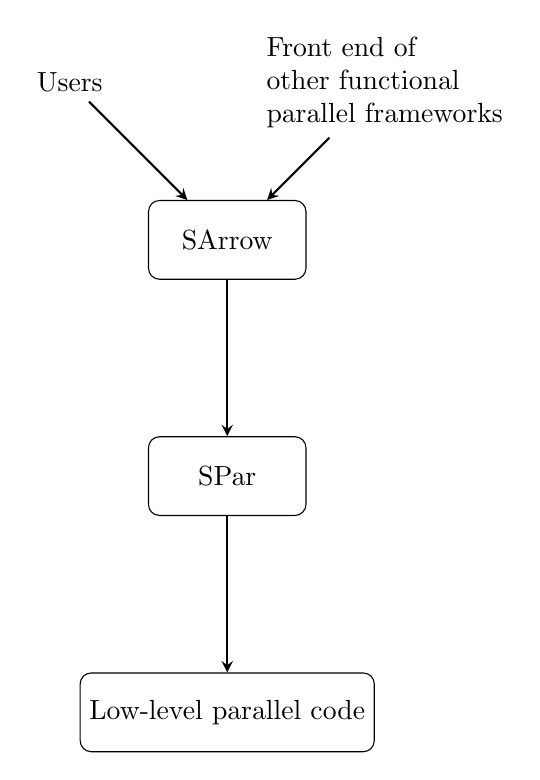
\begin{tikzpicture}[xscale=.5]
    \tikzstyle{proc}  = [rectangle, rounded corners, minimum width=2cm, minimum height=1cm,text centered, draw=black] 
    \tikzstyle{proc1} = [circle,  minimum width=1cm, minimum height=1cm,text centered, draw=black] 
    \tikzstyle{arrow} = [thick,->,>=stealth]
    \node (a) [proc] at (0, 3)  {SArrow};
    \node (b) [proc] at (0, 0)  {SPar};
    \node (c) [proc] at (0, -3) {Low-level parallel code};
    \node (d)  at (-4, 5) {Users};
    \node (e) [align=left] at (4, 5) {Front end of \\ other functional  \\ parallel frameworks};
    \draw[arrow] (a) to (b);
    \draw[arrow] (b) to (c);
    \draw[arrow] (d) to (a);
    \draw[arrow] (e) to (a);
    \end{tikzpicture}
    \caption{Visualization of the workflow}
    \label{intro:fig:workflow}
\end{figure}
The result of project is a embedded high-level framework in Haskell that is capable of generating low-level parallel code. The major contributions are:
\begin{enumerate}
    \item \textbf{Session-typed intermediate language. } We create an intermediate embedded domain specific language (EDSL): SPar: a session typed free monad EDSL for message passing concurrency. This language can be typed by local types, and hence, we can apply multiple results from the multiparty session types to our framework, especially in terms of safety of generated code and reasoning of communication patterns.
    \item \textbf{Intuitive user interface. } One innovation of this project is that we apply the mature Arrow interface for users to express parallel computations. We call the interface SArrow: an arrow interface for writing SPar expressions. It is an abstraction layer on top of SPar, which hides communication primitives from users so that users can express parallel algorithms similar to what they would write for sequential programs.
    \item \textbf{Multiple backends. } We create a backend to generate parallel C code from SPar expressions. The core of the backend is Instr: a low-level EDSL that is independent of target languages. This means that we can support multiple target languages with ease without re-implementing multiple backends. In addition to the code generation backend, we implement an interpreter backend in Haskell for experimenting and fast verification.
    \item \textbf{Evaluations. } Finally, we show the expressive power of the framework by implementing several common computation patterns and three algorithms using our interface. We evaluate the performance of the generated code from the algorithms on high-performance computers as well as PCs. 
\end{enumerate}
The \figref{intro:fig:workflow} summaries the workflow of the framework visually. The main principle supporting the framework is that we convert data flow into communications and from the communication patterns, we gain parallel codes. The results of expressing computation in the framework are 1) compilation to efficient deadlock-free low-level parallel programs and 2) a set of local types to reason the structure of the parallel computation.

At the end of the project, we have discovered two use case of the framework. The primary application is a stand-alone tool to generate parallel C code, and another is a backend for other data-flow based parallel frameworks. 

\section{Report outlines}

\charef{chap:b} gives an overview of the background and related researches. We present the syntax and semantics of SPar in \charef{chap:spar} followed by \charef{chap:impl} introducing the implementation aspect of SPar like session typing and interpreter. \charef{chap:arrow} demonstrates the Arrow interface with examples of parallel patterns formed by the interface and justification of the interface satisfying arrow laws. The discussion about some implementation specific issues like role allocation is also contained in \charef{chap:arrow}. In \charef{chap:cg}, we show the code generation backend and discuss our solutions to challenges when compiling to C, i.e. the problem of representing polymorphic algebraic data structure in C. \charef{chap:eval} explains our benchmarks and shows the performance of the generated code. This chapter can also be regarded as a tutorial on how to use the framework. Finally, we conclude with potential future improvements and remarks on this project. We also include the generated C code in the appendix for curious readers.